\documentclass[journal,twoside]{IEEEtran}
\IEEEoverridecommandlockouts
% The preceding line is only needed to identify funding in the first footnote. If that is unneeded, please comment it out.
\usepackage{cite}
\usepackage{hyperref}
\usepackage{natbib}
\usepackage{booktabs}
\usepackage{threeparttable}
\usepackage{amsmath,amssymb,amsfonts}
\usepackage{algorithmic}
\usepackage{graphicx}
\usepackage{textcomp}
\usepackage{xcolor}
\makeatletter
\def\UrlAlphabet{%
      \do\a\do\b\do\c\do\d\do\e\do\f\do\g\do\h\do\i\do\j%
      \do\k\do\l\do\m\do\n\do\o\do\p\do\q\do\r\do\s\do\t%
      \do\u\do\v\do\w\do\x\do\y\do\z\do\A\do\B\do\C\do\D%
      \do\E\do\F\do\G\do\H\do\I\do\J\do\K\do\L\do\M\do\N%
      \do\O\do\P\do\Q\do\R\do\S\do\T\do\U\do\V\do\W\do\X%
      \do\Y\do\Z}
\def\UrlDigits{\do\1\do\2\do\3\do\4\do\5\do\6\do\7\do\8\do\9\do\0}
\g@addto@macro{\UrlBreaks}{\UrlOrds}
\g@addto@macro{\UrlBreaks}{\UrlAlphabet}
\g@addto@macro{\UrlBreaks}{\UrlDigits}
\makeatother
\def\BibTeX{{\rm B\kern-.05em{\sc i\kern-.025em b}\kern-.08em
    T\kern-.1667em\lower.7ex\hbox{E}\kern-.125emX}}
\pagestyle{headings}
\markboth{Bioinformatics. Specialty  Innovation  and  Entrepreneurship  Training 2021}
{Zhao. A Bayesian Statistics Based Probabilistic Graphical Model for Prediction of Eukaryotic Genetic Splice Sites (June 2021)}
\begin{document}

\title{Bayesian Network: A Bayesian Statistics Based Probabilistic Graphical Model for Prediction of Eukaryotic Genetic Splice Sites\\
}

\author{\IEEEauthorblockN{1\textsuperscript{st} Ziwen Zhao} \\
\IEEEauthorblockA{\textit{College of Life Science and Technology} \\
\textit{Huazhong University of Science and Technology}\\
Wuhan, China \\
justn582@gmail.com}
}

\maketitle

\begin{abstract}
Splice sites are a vitally important gene sequence pattern amongst the functional sites inside a eukaryotic gene. However, splice site prediction does not come easy thanks to the extreme complexity of human genome. In this paper, we use a probabilistic graphical model which considers long range interdependency among nucleotide sequences by learning a direct acyclic graph (DAG), finding all of the conditional probabilities for each of the variables which will be used to search for missing labels of the testing sequences. We discussed several structural learning and parametric learning methods and chose the fittest one with the best type \uppercase\expandafter{\romannumeral1} error found. We evaluated our model with some other approaches on the renowned Kulp \& Reese human genome dataset, during which we found the limitations of its applications and made an analysis and elaboration for Bayesian networks. The source code is available on GitHub and can be obtained from \url{https://github.com/Newiz430/SplicePredictor}. 
\end{abstract}

\begin{IEEEkeywords}
splice site, Bayesian network, direct acyclic graph, PC algorithm, maximum likelihood algorithm, long range interdependency
\end{IEEEkeywords}

\begin{figure}[htbp]
\centerline{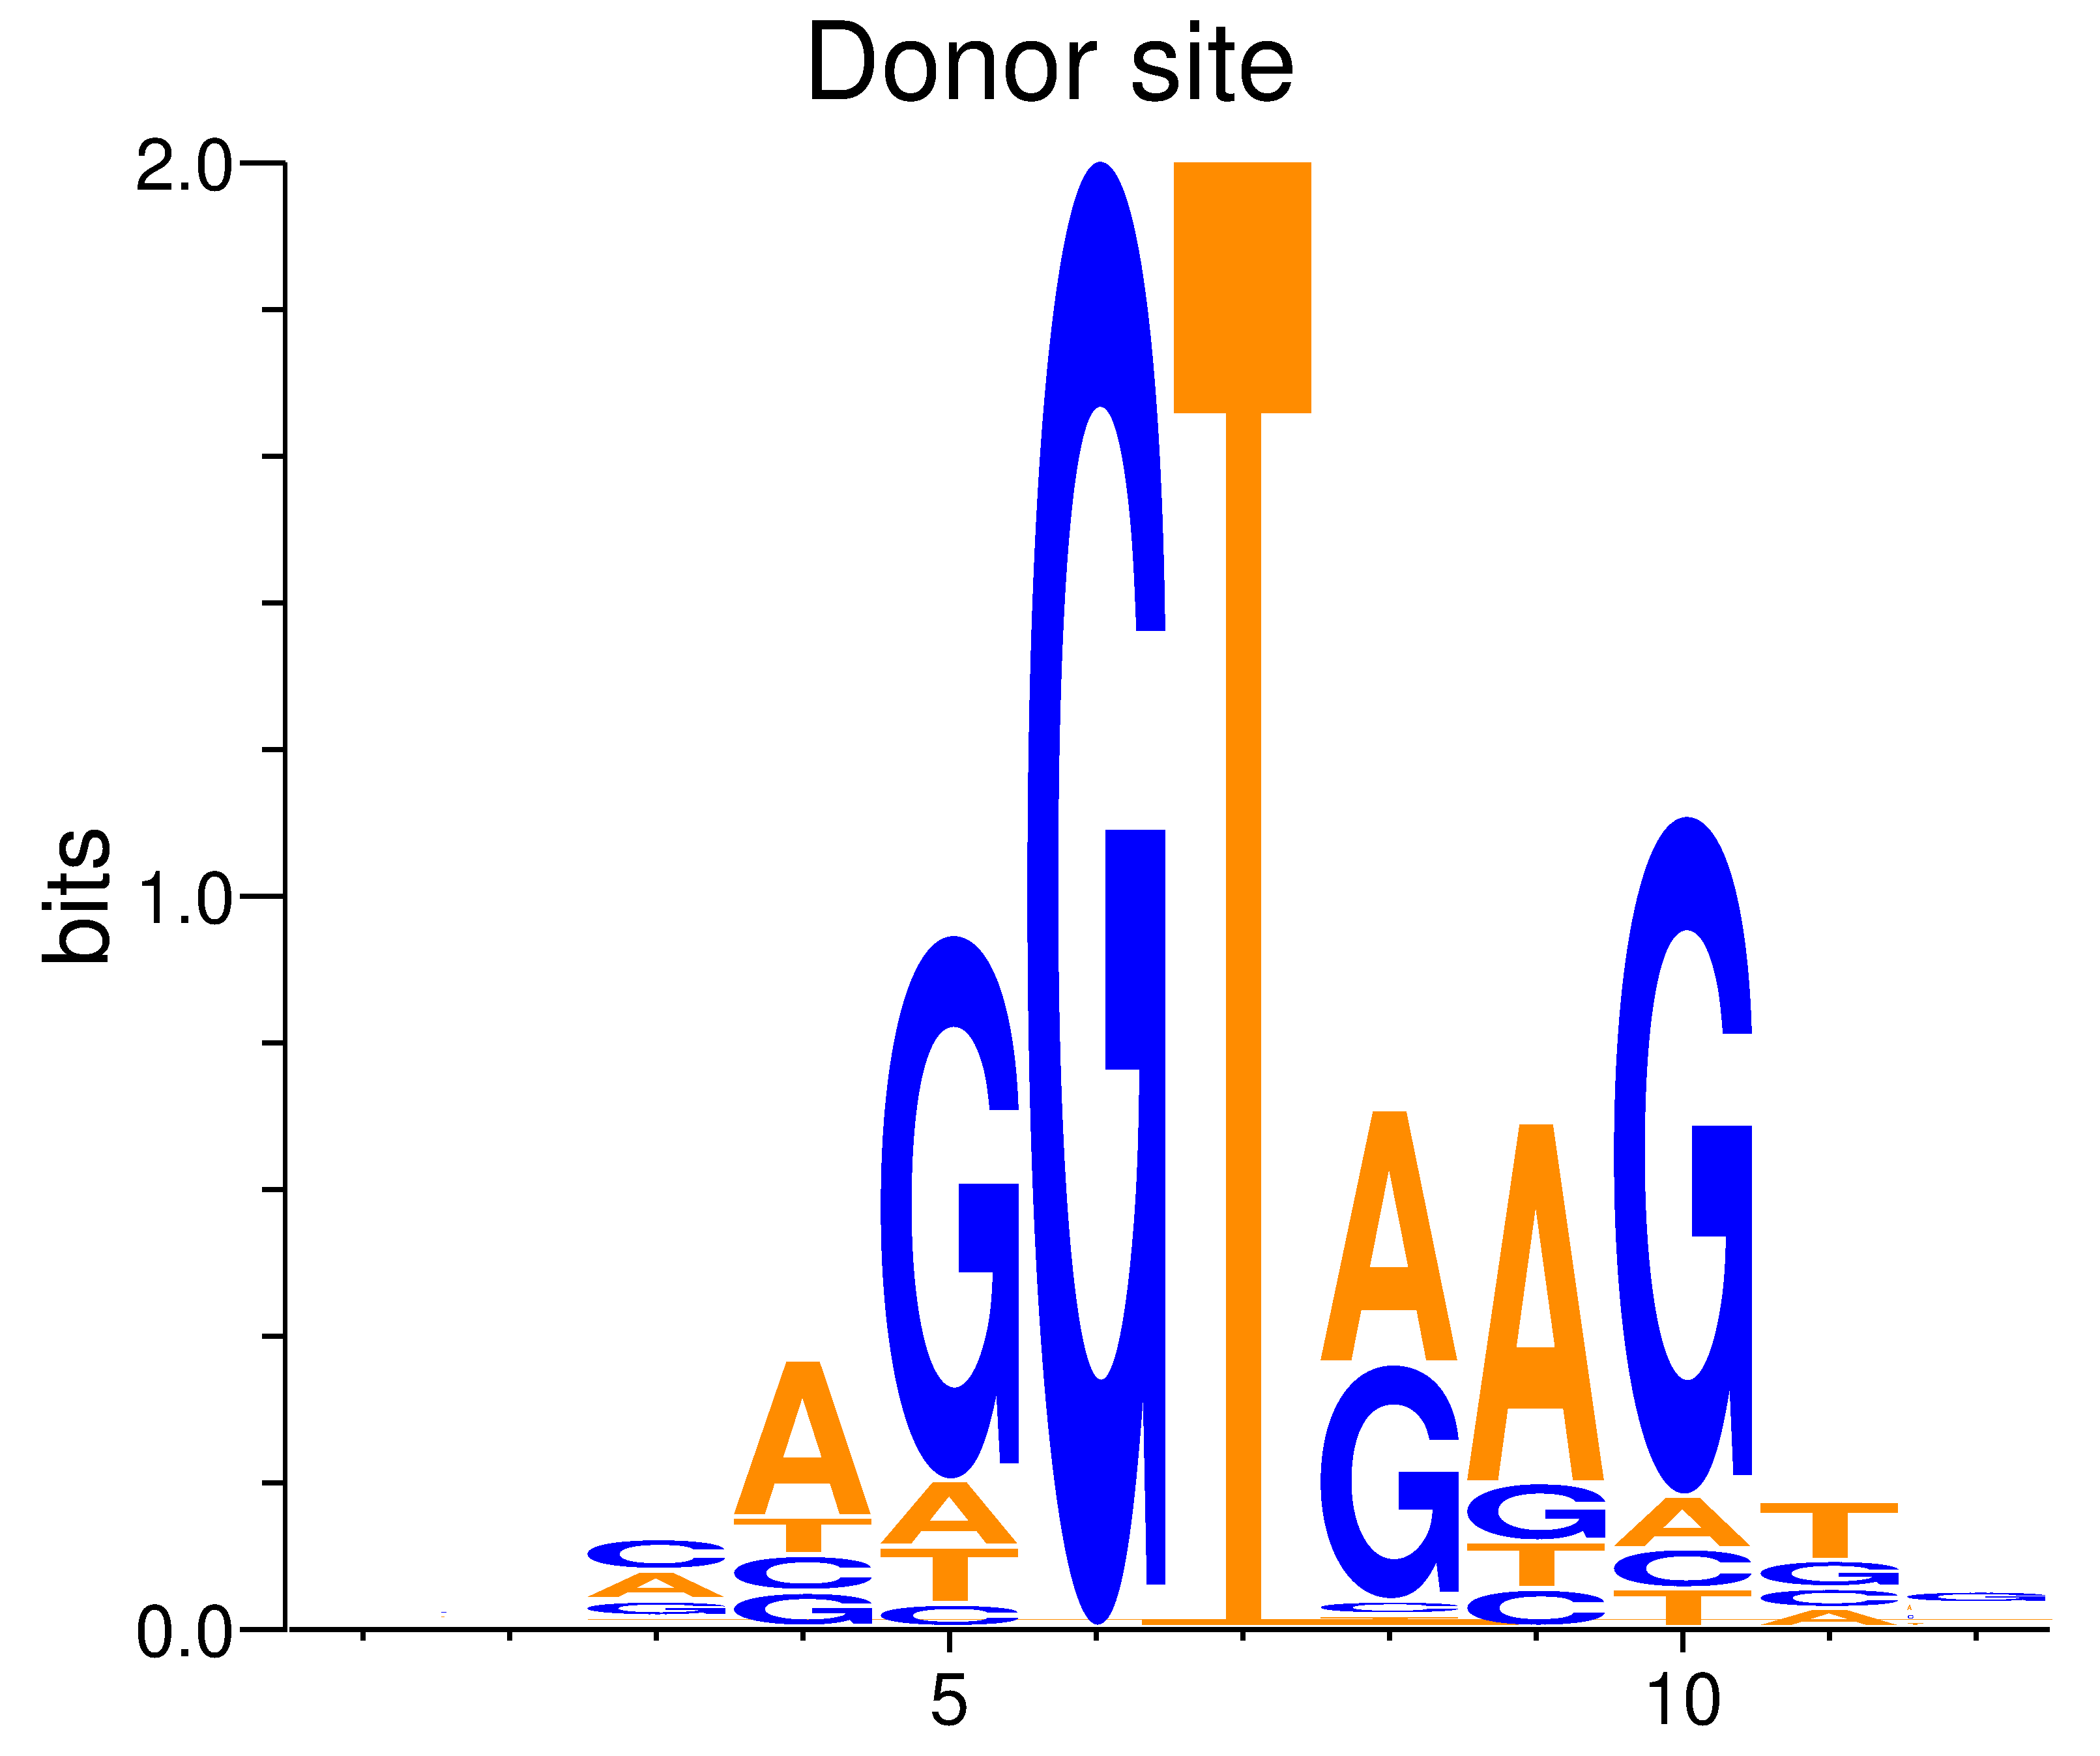
\includegraphics[scale=0.85]{Pics/donor_logo.png}}
\centerline{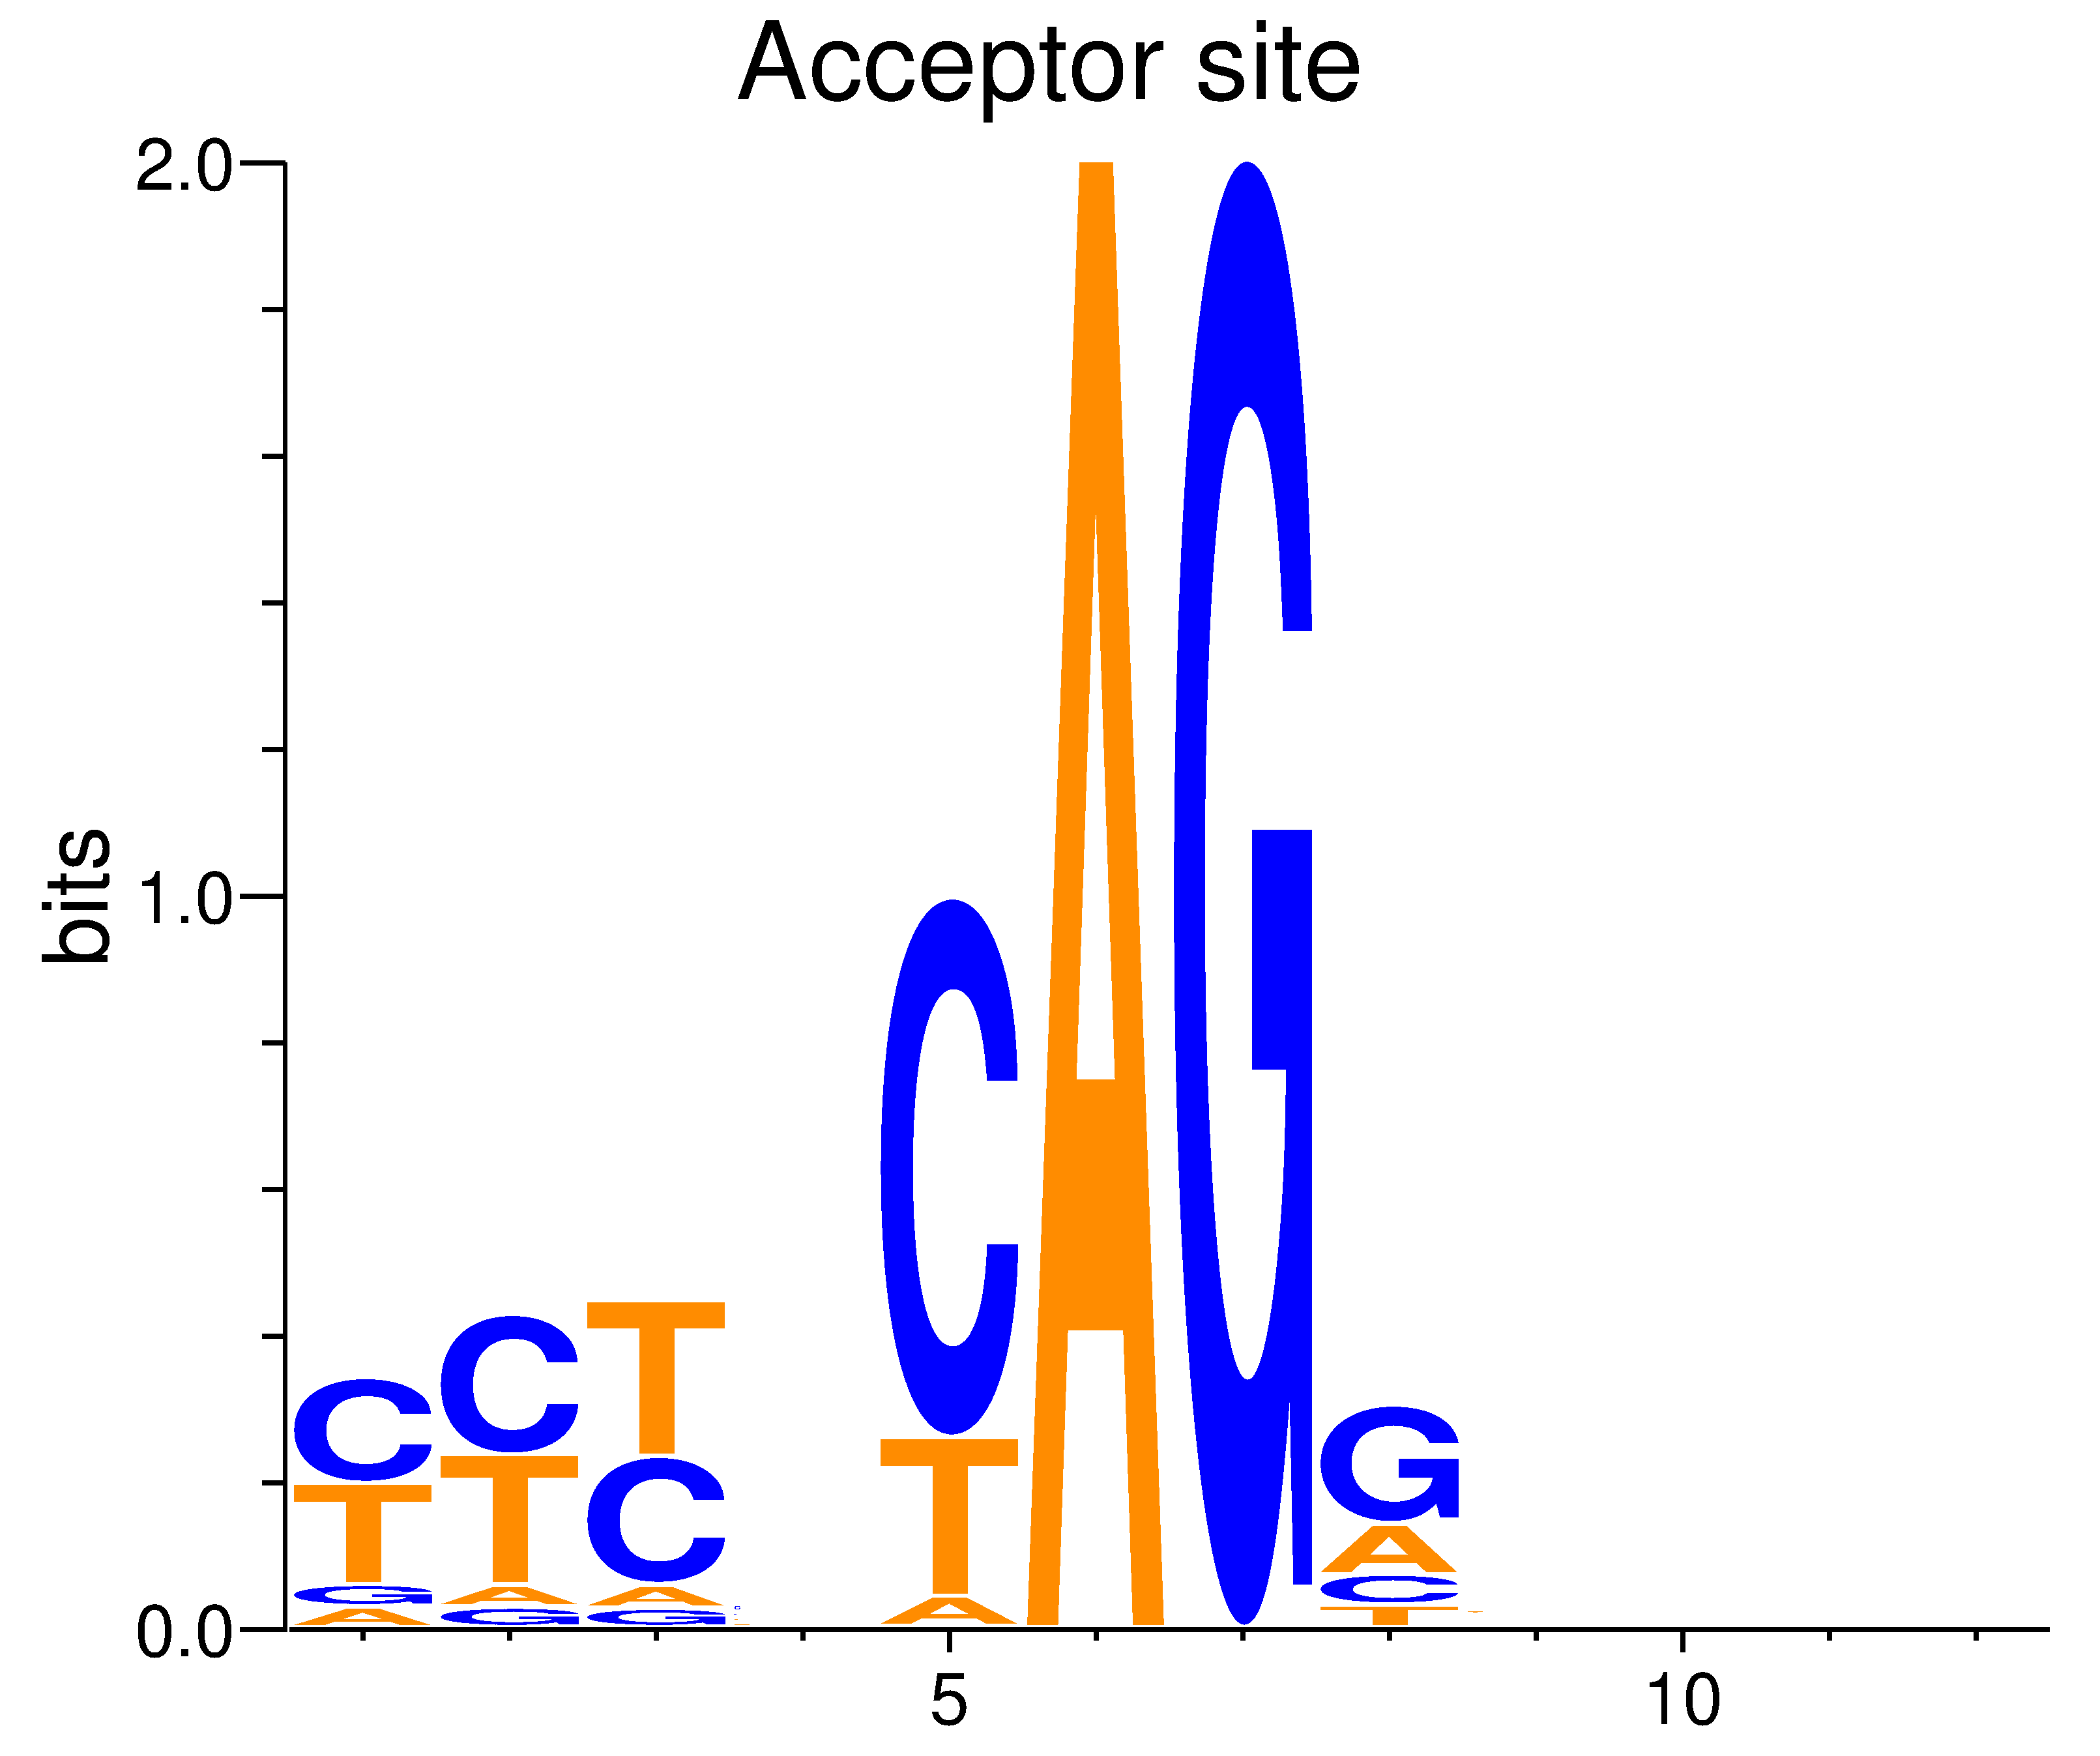
\includegraphics[scale=0.85]{Pics/acceptor_logo.png}}
\caption{Base distribution represented as sequence logos \cite{schneider1990sequence} for eukaryotic gene splice sites (5 upstream sites, 2 conservative sites \& 5 downstream sites): \textbf{top}, donor site; \textbf{bottom}, acceptor site. The most conserved sites is revealed within logo pictures: for donor sites, GT (6, 7); acceptor sites, AG (6, 7). Despite these two, distribution of adjacent sites (5, 8, 9, 10 for the donor, 5 for the acceptor) appear to have some consistency, too. The polypyrimidine tract can also be observed upstream of the acceptor site (1, 2, 3). The information content at a certain point $R_i$ is given by $R_i = \log_24 - (H_i + e_n)$ where $H_i = -\sum\limits_{i=1}^4{P_i(\log_2{P_i})}$ is the Shannon entropy \cite{shannon1948mathematical}, using bit as the basic unit. Higher the bits, higher the relative frequency of that base \cite{schneider1986information}. }
\label{fig1}
\end{figure}

\section{Introduction}\label{1}

\IEEEPARstart{G}{ene} finding by computational methodologies, the foundation for all further investigation in functional genomics, has attracted considerable research attention since the 20\textsuperscript{th} century \cite{burge1997prediction}. With the thriving of functional genomics after the completion of Human Genome Project (HGP), functions of the elements of eukaryotic gene sequences were beginning to surface. Researchers came to realize that DNA sequences, other than genes, contain a huge amount of information, most of which is correlated with the structural features of nucleic acids and in general determines the DNA - protein, or DNA - RNA interactions. Such information is mostly provided by a variety of functional sites (i.e. sequence motif). The splice sites are a vitally important eukaryotic gene sequence pattern amongst all these sites. As terminal points of RNA splicing, splice sites label the junction of transcript exons and introns, assisting biologists in identifying and positioning the coding sequence within a gene. Splicing, itself, also influences the structure and function of genes, which makes genes more ``modular'', allowing new combinations of exons to be created during evolution. Furthermore, new exons can be inserted into old introns, creating new proteins without disrupting the function of the old gene \cite{clancy2008rna}. Hence the discovery and prediction of splice sites are of great significance for genetic selective expression research. 

A splice site locates in the edge of an intron, including a donor site (5' end of the intron) and an acceptor site (3' end of the intron). As a typical sequence motif, the donor site includes an almost invariant sequence GU at the 5' end of the intron, within a larger, less highly conserved region. The splice acceptor site at the 3' end terminates the intron with an almost invariant AG sequence \cite{black2003mechanisms}.  Some sections of the intron foretell the positions of these two sites. For example, a fragment of sequence upstream of the acceptor consisting of cytosines and thymines, which is called a polypyrimidine tract \cite{lodish2008molecular}. Fig. \ref{fig1} shows the base distributions adjacent of the splice donor sites and acceptor sites. 

As a matter of fact, accurate prediction does not come easy thanks to the extreme complexity of human genome. On one hand, the number and length of exons and introns in a eukaryotic gene exhibit great uncertainty. One eukaryotic gene contains 5.48 exons with 30 - 36 bps long on average. While the longest exon in the human genome is 11555 bp long, several exons have been found to be only 2 bp long \cite{sakharkar2004distributions}. On the other, the existence of alternate splicing make it harder to predict \cite{black2003mechanisms}. In this paper, we apply a Bayesian method for gene functional site finding to predict eukaryotic gene splice sites, and prove its feasibility. 

\subsection{Related Work}\label{1.1}

Several typical computational methods that attempt to predict eukaryotic splice sites from unknown gene sequences (i.e. \textsl{ab initio} prediction) have been proposed previously. 

Frequency-based methods count the nucleotide frequencies of each site via multiple sequence alignment, etc. and work out the log-odds ratio to compare and find conservative sections in the alignment results. Rodger, et al. (1983) \cite{staden1984computer} proposed a computational model using a weight matrix to represent each type of recognition sequence. A weight matrix is a two dimensional array of values that represent the score for finding each of the possible sequence characters at each position in the target signal. The Weight Matrix Model (WMM) now becomes deprecated owing to its poor accuracy and its independence assumption, that is, WMM only takes point-wise base distribution into consideration, regardless of the potential dependence between adjacent points which is more conformable to the realistic situations. Zhang et al. (1993) \cite{zhang1993weight} optimized the weight matrix to weight arrays which take into account the correspondence between current position and an adjoining position, which is certified conducive to promote accuracy of splice site prediction, but this is still relying on the hypothesis that the intrinsic interdependency only exists between adjacent sites. To deal with the predicament, Burge, et al. (1997) \cite{burge1997prediction} explored a maximal dependence decomposition method and developed the software GENSCAN which identifies complete exon / intron structures of genes, which performs better but still generates many false positive results. 

Supervised learning methods learn a model from existing training set which is able to identify the most effective pattern automatically. Duan, et al. (2008) \cite{duan2008position} developed the support vector machine (SVM) for position-specific residue preference feature prediction which determines the second structure of double helices. Ryen et al. (2008) \cite{ryen2008splice} introduced the artificial neural network (ANN) in this area and trained the model with backpropagation, which can make predictions without prior knowledge of any sensor signals. Accurate and efficient learning approaches they are, supervised learning methods are heavily dependent on the mass and quality of training sets. Models may not be improved and a computational resource waste may happen when an unbalanced dataset or one with too many noises is provided. For SVMs, kernel function selection is a tricky problem, and neural networks acquire a suitable framework and initial hyperparameters. 

\subsection{Contributions}\label{1.2}

In this work, we use a probabilistic graphical model which considers long range interdependency among nucleotide sequences by learning a direct acyclic graph (DAG), finding all of the conditional probabilities for each of the variables which will be used to search for missing labels of the testing sequences. Our contributions are listed as follows. 

\begin{itemize}
\item We implemented the Bayesian network by Pgmpy, Python \cite{ankan2015pgmpy} using the given KR set and estimated its performance on the BG set, referring to the existing experiment by Chen, et al. (2005) \cite{chen2005prediction}
\item We assessed the influence of different type \uppercase\expandafter{\romannumeral1} errors on the construction of DAG and performance on the given dataset. 
\item We did a comparison study among WMM, WAM, 3 kinds of SVM and our network to show the performance (also limitations) of Bayesian networks. 
\end{itemize}

\begin{figure*}[htbp]
\centerline{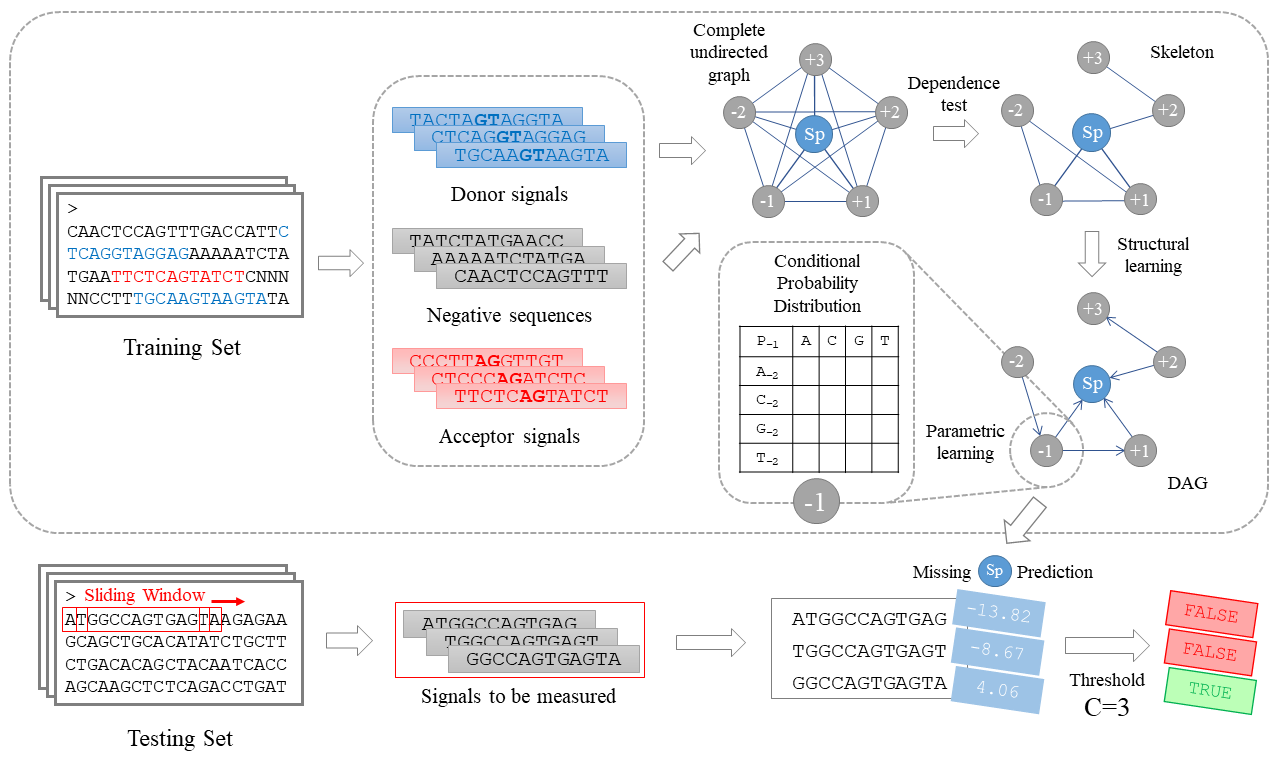
\includegraphics[scale=0.5]{Pics/BN.png}}
\caption{Overall architecture of the Bayesian network splice predictor. Taking the PC Algorithm \cite{spirtes1991algorithm} as an example, we use the training set to learn a network by the following steps: extracting positive site signals \& randomly choosing negative signals, creating a complete undirected graph first, removing edges by dependency tests, orienting edges to form a DAG, and create condition probability distribution (CPD) tables for each node \cite{neapolitan2004learning}. This network is used to predict unknown signals by these steps: extracting testing sequences of same length by window-sliding, scoring the sequences position-wise by computing the conditional probability of the missing label node `Sp', calculating the binary log-odds scores, and comparing them with a given threshold to make final judgment. }
\label{fig2}
\end{figure*}

\section{Methods}\label{2}

Our method is illustrated in Fig. \ref{fig2}, which mainly contains three parts. A DAG structure is learned from the training data during the ``structural learning'' step, the conditional probability frames of variables are calculated during the ``parametric learning'' step and sequences of the testing set are scored by the network at the ``predicting'' step. See below for more detailed presentation. 

\subsection{Hypothesis}\label{2.1}

We assume conservation around the functional splice sites through the entire experiment. This is the fundamental premise for fundamental site finding methods. As for data, we assume that everything about the splice site pattern remained unknown (including the obligatory sites GT / AG) until we dug them out, in order to guarantee the generality of our model, since our aim is to make it possible to branch out to other unidentified functional sites. 

\subsection{Data Extraction}\label{2.2}

Dash et al. (2001) \cite{dash2001modeling} found in predicting splice sites by a Bayesian network that it achieves better performance when both of the upstream and downstream feature lengths are greater than 15. With a view to simplifying model and decreasing the computation, we choose 5 upstream sites and 7 downstream sites of intron / exon junctions to form 12 nt long signal sequences from the primary training set. We abandon sequences containing ambiguous bases, whose correspondence with the splice sites we consider inapparent. The training set provides 2,381 donor signals and 2,381 acceptor signals. As for negative samples, Chen, et al. \cite{chen2005prediction} used pseudo splice sites as false data, extracted by searching for negative sample sequences with $P_{+1}P_{+2} = \text{GU / AG}$ whereas, according to the splice site hypothesis above, We randomly selected about 5,000 sites in sections which do not intersect with all donor and acceptor sites, and combined with positive ones to get actual training dataset, the positive-negative ratio of which is about 1:2. Additionally, we export sequences with the same length by window sliding from the primal testing set and build the actual testing set in a positive-negative ratio of 1:20. 

For the data imbalance of negative sites versus positive ones, a feasible approach was proposed by Wen, et al. (1999) \cite{fang1999splice} who split the SVM classifier into 3 sub-classifiers which use a shared set of positive samples but different sets of negative samples, and picked the lowest prediction score on the testing set among all 3 scores generated by sub-classifiers as the final result. Instead we simply used the oversampling strategy, as we made a copy of the positive sites to expand the positive sample size up to 4,762 sequences, which converts the positive-negative ratio into about 1:1. 

\subsection{Structural Learning}\label{2.3}

For Bayesian network structure building, experts are usually needed for confirming the dependency of variables. For certain of tasks, however, this could be extremely difficult considering the massive time cost and complicated correlation between long range sites. Experts as they are, such interdependency is unlikely to be given explicitly in splice site prediction tasks without the help of existing research findings. Thus it is of great importance to learn a dedicated structure for the Bayesian network via the given data, because what we expect is the dependency between every nodes can be directly mined from statistical training data, instead of the guidance of experts. As a matter of fact, the learning methods indeed exist. We considered two structure learning algorithms with different principles. 

\emph{Scoring \& Searching.} Two parts constitute the scoring \& searching based structure learning approaches. To start with, an appropriate scoring criterion should be selected which assigns a value to each DAG (or DAG pattern) under consideration based on the data \cite{neapolitan2004learning}. The most common scoring functions include Bayesian Dirichlet Scores (BDeu, K2) and Bayesian Information Criterion (BIC) \cite{koller2009probabilistic}. 

\begin{figure*}[htbp]
\centerline{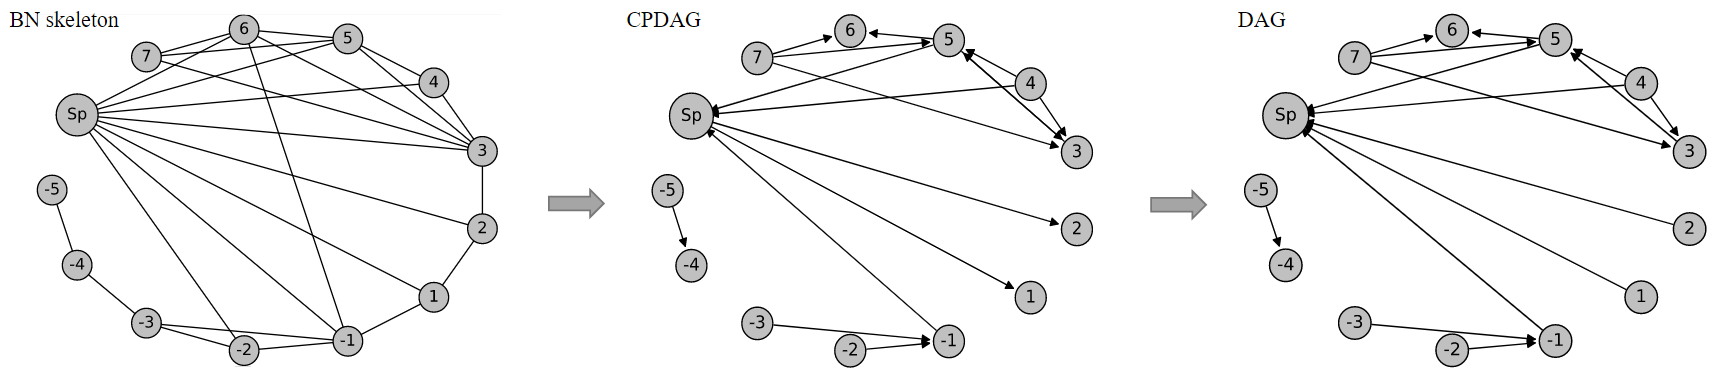
\includegraphics[scale=0.29]{Pics/network.png}}
\caption{How a Bayesian network structure is learned by constraint-based statistical analysis. After we gain the skeleton - also called a dependency graph - by chi-square tests (network on the left), we orient part of some edges by d-separation judgment to form a complete partial DAG. Now we have a network with mostly oriented edges and several undirected edges (labeled with bi-directional arrows in the graph, e.g. $3 \leftrightarrow 5$ in the middle) which we have to cope with. We transform our CPDAG into a DAG (network on the right) by orienting these edges and doing some corrections. The networks are generated during our experiment, with type \uppercase\expandafter{\romannumeral1} error $\alpha = 10^{-5}$. }
\label{fig3}
\end{figure*}

The following model searching consists of determining and selecting the DAG patterns with maximum probability conditional on the data (There could be more than one maximizing DAG pattern in general) \cite{neapolitan2004learning}. For complex DAGs, exhaustive searching is not recommended since it costs a large amount of time to find the global optimum. Hill-climb searching \cite{tsamardinos2006max} heuristically searches for a local optimum by adding and removing a single edge, which performs at a way higher speed but is too greedy to find the global optimum point. Our experiment shows that DAG structure learned by hill climbing is way too complicated (only a few edges are deleted from the complete graph) which consumes unacceptable time for parametric learning and prediction, so this method is also excluded. 

\emph{Constraint Statistical Analysis.} We choose this approach to learn a Bayesian network. Fig. 3 shows how it is done by operating an initial \textsl{complete undirected graph} of base position variables. Other than that, independencies of samples are needed for this structure learning approach. Here we use a chi-squared hypothesis test \cite{pearson1900x} to find out whether a node $u$ is independent from another node $v$, given a set of variables. Next we just remove the edges connecting independent nodes of the complete undirected graph to build a \textsl{skeleton}. 

Because of the causality between two related variables, the edges require orientation and decyclization to change a skeleton into a \textsl{DAG}. Firstly we confirm part of some edges' directions by d-separation judgment, turning the skeleton into a \textsl{complete partial DAG} (CPDAG) \cite{kalisch2007estimating}. This is called a PC algorithm for DAG pattern finding  \cite{spirtes1991algorithm}\cite{neapolitan2004learning}. Then the CPDAG is expanded to a DAG if it is DAG-faithful, which means no more v-structures will be introduced during the expansion. See \cite{neapolitan2004learning} for more details of PC algorithm. 

Our splice site predicting Bayesian network is built by a slightly different way. (1) Aside from the positions of signal sequences, we also add a label node `Sp' which indicates the state of each signal by Trues and Falses. (2) Since `Sp' is dependent on the base distribution of other position nodes, it is reasonable to set the out-degree of `Sp' to zero, thereby we reverse the arrows pointing to it manually (Fig. \ref{fig3}). 

\subsection{Parametric Learning}\label{2.4}

As a DAG structure is not able to assist directly in predicting hidden splice sites in the genomic DNA sequence, parametric learning of the Bayesian network is acquired to obtain the conditional probability distributions for each state of every node. Two approaches are proposed for parametric learning. 

Heckerman, et al. (1998) \cite{heckerman2008tutorial} proposed a maximum likelihood algorithm for network learning: let $\theta$ be the CPD of $V_A$ given the parents $V_{P_i} (i = 1, 2, \cdots)$, the learning process searches for a perfect $\theta$ s.t. the summation of $P(V_A | V_P, \theta)$ for all parents reaches the top. To this end, the algorithm computes the state counts $\text{freq}(V_A = N)$ and divides each cell by the (conditional) sample size $\text{freq}(V_{P_i} = M_i)$ \cite{koller2009probabilistic}. $\theta$ is filled with conditional probabilities given by:

\begin{multline}
P(V_A = N \ | \ V_{P_1} = M_1, V_{P_2} = M_2, \cdots) \\
= \displaystyle\frac{\text{freq}(V_A = N, V_{P_1} = M_1, V_{P_2} = M_2, \cdots)}{\text{freq}(V_{P_1} = M_1, V_{P_2} = M_2, \cdots)}
\label{eq1}
\end{multline}
\begin{equation}
P_0(V_A = N) = \displaystyle\frac{\text{freq}(V_A = N)}{\sum\limits_N \text{freq}(V_A = N)}
\label{eq2}
\end{equation}
where $P_0(V_A = N)$ is the initial probability for nodes with in-degree = 0. 

Since the maximum likelihood algorithm may cause overfitting with lack of data, Bayesian Parameter estimating algorithm is introduced. The premise of Bayesian estimation is the prior distribution of each site to be known. These distributions act as pseudo-counts in the Laplace smoothing method \cite{schutze2008introduction} and are added to the actual state counts \cite{koller2009probabilistic}. 

\begin{figure*}[htbp]
\centerline{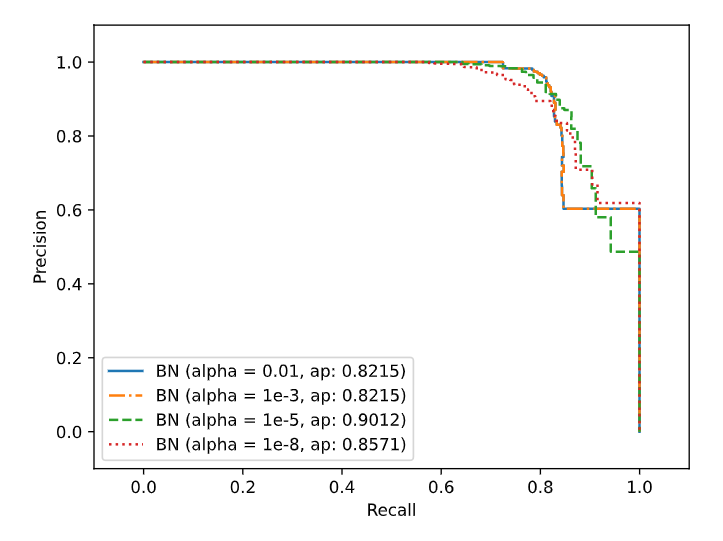
\includegraphics[scale=0.35]{Pics/bn_prcurve.png}
    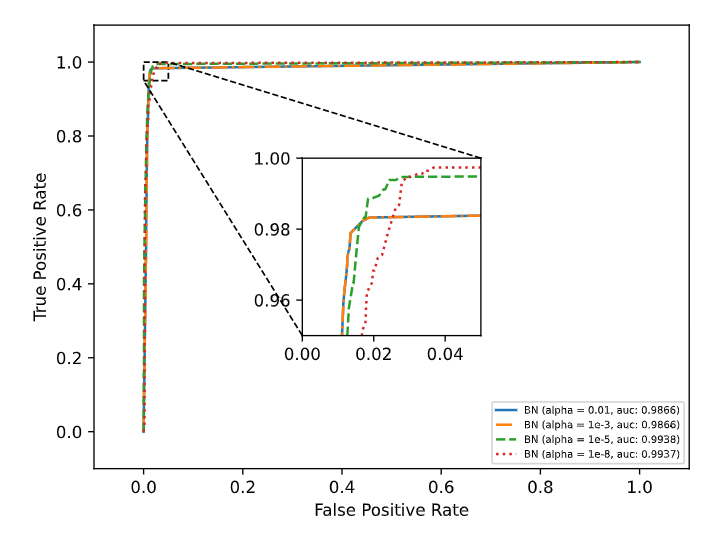
\includegraphics[scale=0.35]{Pics/bn_roccurve.png}}
\caption{Performance of BN models with different type \uppercase\expandafter{\romannumeral1} error settings on the KR set. \textbf{Left}, P-R curves for comparison. Research shows that BN with type \uppercase\expandafter{\romannumeral1} error $\alpha=10^{-5}$ outperforms the other models, with the average precision surpassing the runner-up 0.044. This implies that $\alpha=10^{-5}$ does a great tradeoff between the correspondence and independency of position vertices. However, BNs with $\alpha=0.01$ and $\alpha=10^{-3}$ learn noisy dependencies and misclassify some positive samples with very low scores, so false positive samples rise sharply only when Recall is about 0.8. \textbf{Right}, ROC curves for comparison. BN with $\alpha=10^{-8}$ shows a very close performance to the best model compared by AUC values, which means that it has also learned the essential correlations of long range positions. }
\label{fig4}
\end{figure*}

\begin{figure*}[htbp]
\centerline{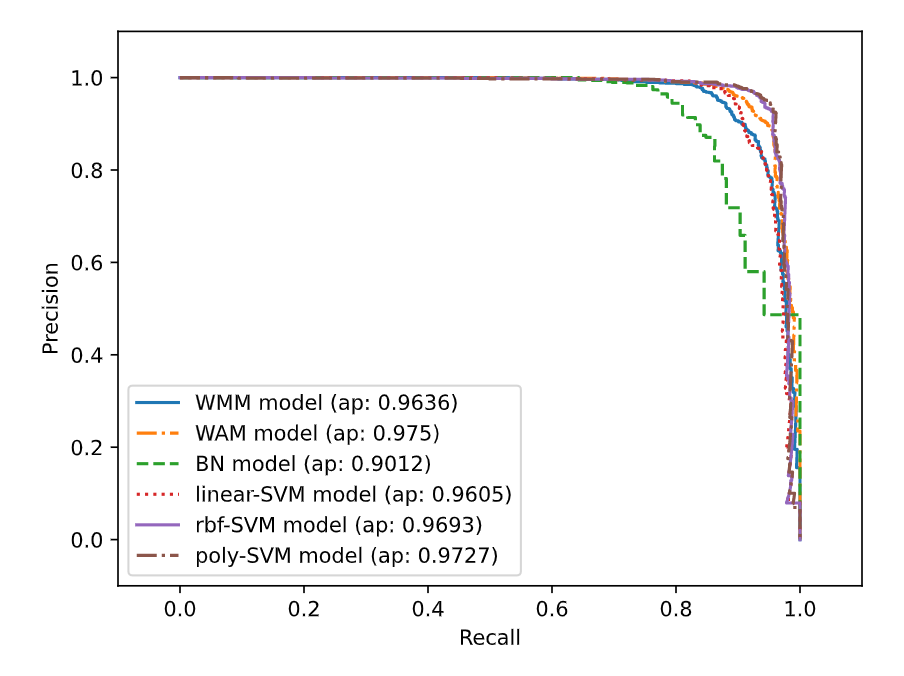
\includegraphics[scale=0.28]{Pics/all_prcurve_donor.png}
    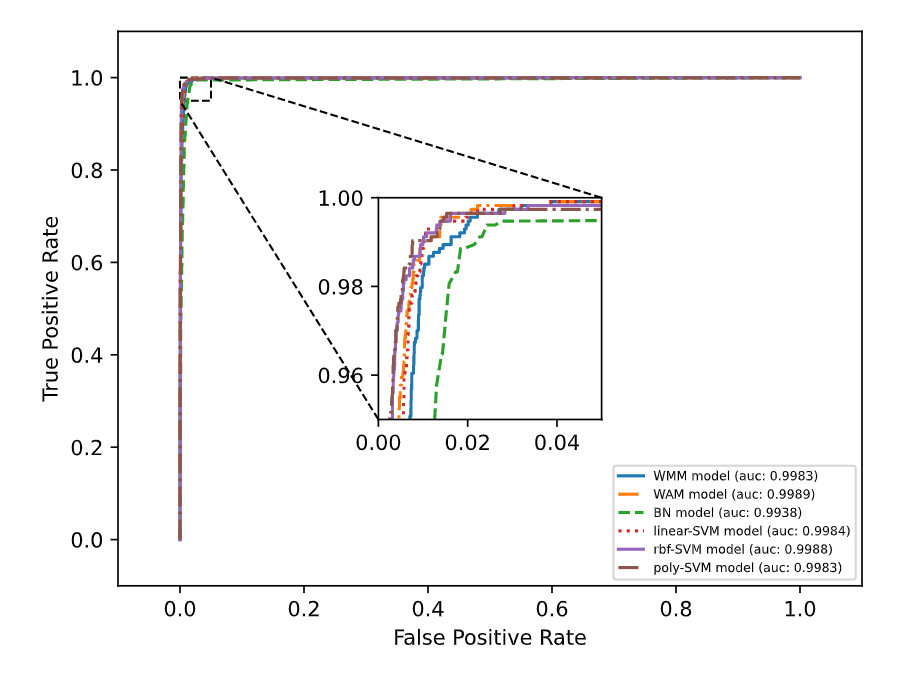
\includegraphics[scale=0.28]{Pics/all_roccurve_donor.png}}
\caption{Overall comparison of splice predictors on a balanced KR set. \textbf{Left}, P-R curves which show an abnormal comparison result of Bayesian model performance. Even the BN with the best $\alpha = 10^{-5}$ performs the worst among all models, which is unacceptable considering its huge amount of predicting time cost. \textbf{Right}, ROC curves, where the AUC of BN show a -0.004 less than the simplest predictor. This may be explained by the simplicity of splice site patterns: models need to pay more attention on the short range correlations instead of long ones in predicting splice sites. Models considering short correlations only perform better (with WAM reaching the top, unexpectedly), which also proves our explanation. }
\label{fig5}
\end{figure*}

\subsection{Prediction}\label{2.5}

The last part of our work is that we use the completed network to perform statistical inference on the testing data. Above all, the extracted testing data (by a sliding window) is preprocessed by dropping the columns which are conditionally independent of all the other positions according to the network structure (sometimes separated vertices appear in the network which is considered weakly-related to the other variables), that is, useless for splice site prediction. We calculate posterior probabilities $P(V_{Sp} = \text{True})$ using the condition probabilities provided by $\theta$s that is:
\begin{small}
\begin{align}
P(V_{Sp} = \text{True}) & = \sum\limits_{M_1, M_2, \cdots}\!\!\!\!P(V_{Sp} = \text{True}, V_1 = M_1, V_2 = M_2, \cdots) \notag \\
& = \sum\limits_{M_1, M_2, \cdots}\!\prod\limits_{i, j} P(V_i = M_i \ | \ V_j = M_j), \notag \\  
& \text{if} \ V_j \rightarrow V_i \ \text{exists}.
\label{eq3}
\end{align}
\end{small}
In this way, we score the extracted data with the log-odds function $S(X)$: 
\begin{equation}
S(X) = \ln \displaystyle\frac{P(V_{Sp} = \text{True})}{P(V_{Sp} = \text{False})}
\label{eq4}
\end{equation}

Since the posterior probabilities may contain zeros created by the CPD product, we set $P = 10^{-6}$ to avoid division-by-zero error which, in the meantime, guarantees a higher penalty for a sequence including a $P(V_{Sp} = \text{True}) = 0$ site, and vice versa. 

Transformation from scores to predicting results needs the comparison. We can filter the true positive sites we need from batches of scores by taking different thresholds. It is necessary to exercise caution in selecting the threshold $C$. A large $C$ will exclude potential positive sites, while a small $C$ misclassifies negative sites as positive. Hence an appropriate threshold is a tradeoff based on the specificity and sensitivity of a model. For the threshold optima selection, see \ref{4} for details. 

\section{Experiments}\label{3}

\subsection{Data}\label{3.1}

We conduct our experiment on the eukaryotic gene sequence dataset Kulp \& Reese \cite{reese1997improved} and Burset \& Guigo \cite{burset1996evaluation}. Human genome sequence dataset Kulp \& Reese (KR set) is used as training set which contains 462 sequence text files, each records the name, length, CDS terminal points and the segment. 2,381 donor sites and 2,381 acceptor sites are extracted from the KR set, which are doubled to 4,762 sequences for balancing. Vertebrate genome dataset Burset \& Guigo (BG set) is used as testing set which contains 570 sequence text files with a similar format, except for a lack of the sequence length. 

The KR and BG set is open access and you can get the entire dataset at \url{https://www.fruitfly.org/sequence/human-datasets.html} and \url{http://www1.imim.es/databases/genomics96/}. 

\subsection{Metrics}\label{3.2}

Our model accuracy measures are given by \eqref{eq5} -- \eqref{eq11}: 
\begin{gather}
    \text{Precision} = \displaystyle\frac{\text{TP}}{\text{TP} + \text{FP}}\label{eq5} \\
    \text{Recall} = \displaystyle\frac{\text{TP}}{\text{TP} + \text{FN}}\label{eq6} \\
    \text{FPR} = \displaystyle\frac{\text{FP}}{\text{TN} + \text{FP}}\label{eq7} \\
    \text{TPR} = \displaystyle\frac{\text{TP}}{\text{TP} + \text{FN}}\label{eq8} \\
    \text{F1-Score} = \displaystyle\frac{2 \times \text{Precision} \times \text{Recall}}{\text{Precision} + \text{Recall}}\label{eq9}
\end{gather}
where $\text{TP}$, $\text{FP}$, $\text{TN}$, $\text{FN}$ are metrics of the confusion matrix \cite{stehman1997selecting}. Precision-Recall curves and ROC curves \cite{powers2020evaluation}\cite{fawcett2006introduction} are plotted to make the performance of our model more intuitive. We also calculate areas under the curves by: 
\begin{gather}
    \text{AP} = \int_0^1 P(R)\text{d}R = \sum\limits_{i=1}^n P_i\Delta R_i\label{eq10} \\
    \text{AUC} = \int_0^1 T(F)\text{d}F = \sum\limits_{i=1}^n T_i\Delta F_i\label{eq11}
\end{gather}
where $\text{AP}$ summarizes a precision-recall curve as the weighted mean of precisions achieved at each threshold, with the increase in recall from the previous threshold used as the weight \cite{zhu2004recall}. $\text{AUC}$ is equal to the probability that the model will rank a randomly chosen positive sample higher than a randomly chosen negative one (assuming that "positive" ranks higher than "negative"), where $F$ denotes false positive rate and $T$ denotes true positive rate \cite{fawcett2006introduction}. 

\subsection{Environmental Settings}\label{3.3}

Throughout our experiments, the PC algorithm and maximum likelihood method are used respectively for structural and parametric learning. Chi-squared test is chosen for independence hypothesis testing. We use the parallel version of stable PC with multiple threads in order to promote the efficiency of Bayesian network learning. The maximum conditional variables is set to 5 to prevent a runaway growth of CPD size. 

\subsection{Implementation}\label{3.4}

We encapsulate the Bayesian network model in the class \texttt{BayesNet} which is derived from the base class \texttt{Base} in \texttt{`./Model/basemodel.py}. Sequences are extracted by \texttt{./Utils/extract.py} and saved temporarily in an \texttt{Sequence} object. All of the statistical graphs involved in this paper are drawn by the scripts in \texttt{./Utils} using Matplotlib \cite{Hunter:2007}, NetworkX \cite{hagberg2008exploring} \& Weblogo, and saved in \texttt{./Pics}. We evaluate the model using Scikit-Learn for confusion matrices, precision-recall pairs and FPR-TPR pairs \cite{pedregosa2011scikit}. These tools saved considerable time for model training and prediction. Models can be easily saved or loaded by methods \texttt{save\_model()} and \texttt{load\_model()}. All the components have their corresponding interface methods provided in the aforementioned classes. For the code implementation details of Bayesian network, see \texttt{./Model/bn.py}. 

Training \& Predicting process is operated by Ubuntu 18.04.5 LTS on 16 CPU cores with 2 threads each. The source code is available on GitHub and can be obtained from \url{https://github.com/Newiz430/SplicePredictor}. 

\section{Results}\label{4}

\subsection{Type \uppercase\expandafter{\romannumeral1} Errors}\label{4.1}

Type \uppercase\expandafter{\romannumeral1} error is commonly used in chi-squared hypothesis tests which denotes the rejection of a true null hypothesis \cite{dekking2005modern}, i.e. two variables are dependent of each other. The judgment of conditional independency between two sites is influenced by the value of type \uppercase\expandafter{\romannumeral1} error, so does the structure of DAG. Distinct structures of DAGs affect the quality and efficiency of prediction. 

We choose 4 values of type \uppercase\expandafter{\romannumeral1} error $\alpha = 0.01$, $10^{-3}$, $10^{-5}$, $10^{-8}$ for chi-squared test from the PC algorithm and evaluated the model behaviors. Results are shown in Fig. \ref{fig4} and Table \ref{tab1}. Note that BNs with $\alpha=0.01$ by default and $\alpha=10^{-3}$ are nothing like as good as ones with lower $\alpha$s, including the tedious prediction and poor precision. It seems that a higher acceptance of the true null hypothesis would lead to futile learning of numerous useless or noisy edges and massive computation of posterior probabilities, which doubles the decline of model performance. Instead, BNs with $\alpha=10^{-5}$ by default and $\alpha=10^{-8}$ are ideal predictors which achieve higher accuracy with a relatively small time cost. 

\begin{table}[htbp]
\begin{center}
\begin{threeparttable}
\caption{Time Cost of BNs with Different Type \uppercase\expandafter{\romannumeral1} Error Settings}
\begin{tabular}{ccc}
\toprule
Type \uppercase\expandafter{\romannumeral1} Error & Training Time (\times10\textsuperscript{3}s) & Predicting Time (h) \\
\midrule
0.01 & 7.37 & 5.22 \\
1e-3 & 5.02 & 5.27 \\
1e-5 & 3.87 & 1.23 \\
1e-8 & \textbf{0.893} & \textbf{1.13} \\
\bottomrule
\end{tabular}
\label{tab1}
\end{threeparttable}
\end{center}
\end{table}

\begin{figure}[htbp]
\centerline{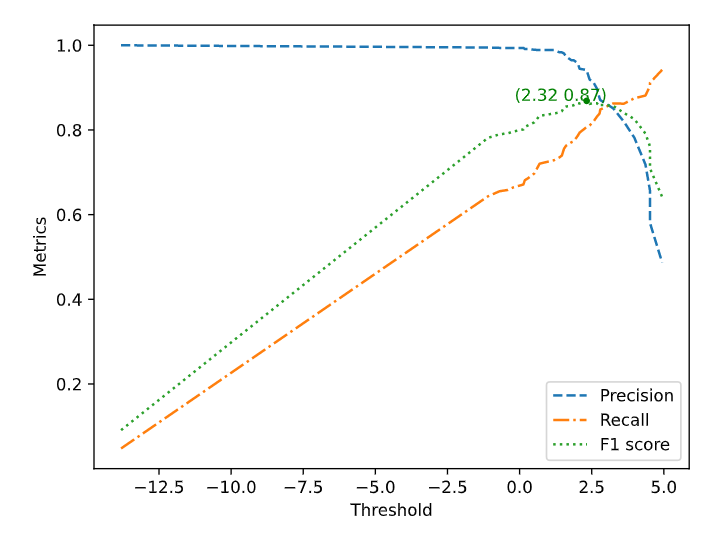
\includegraphics[scale=0.35]{Pics/BN_threshold_donor.png}}
\caption{Searching for the best threshold for donor prediction. F1-score \eqref{eq9} is a balanced metric between precision and recall which expresses best performance of models. We have found the maximum F1 point for BN: (2.32, 0.87). }
\label{fig6}
\end{figure}

\begin{table*}[htbp]
\begin{center}
\begin{threeparttable}
\caption{Performance of BN Against Other Donor Site Predictors\tnote{1}}
\begin{tabular}{lccccc}
\toprule
Method & Precision & Recall (TPR) & FPR & F1-score & Run time(s) \\
\midrule
WMM (threshold = 2.26) & 0.8503 & \textbf{0.9697} & 0.0085 & 0.9061 & \textbf{1.6614} \\
WAM (threshold = 3.09) & 0.9006 & 0.9543 & 0.0053 & 0.9267 & 1.7940 \\
Linear - SVM\tnote{2} (threshold = 1.63) & 0.8801 & 0.9678 & 0.0066 & 0.9219 & 2.3974 \\
RBF - SVM\tnote{2} (threshold = 2.94) & 0.9265 & 0.9278 & 0.0037 & 0.9272 & 3.4894 \\
4D poly - SVM\tnote{2} (threshold = 3.00) & \textbf{0.9290} & 0.9384 & \textbf{0.0036} &  \textbf{0.9337} & 3.0368 \\
BN (threshold = 2.32) & 0.8067 & 0.9410 & 0.0113 & 0.8688 & 4.23e+3 \\
\bottomrule
\end{tabular}
\begin{tablenotes}
    \footnotesize
    \item[1] The argmax thresholds are assigned to these models to get the best metrics. Run time represents the seconds cost in the predicting step. Same for tables below. 
    \item[2] ``Linear - SVM'', ``RBF - SVM'', ``4D poly - SVM'' are support vector machine approaches with different kernels. 
\end{tablenotes}
\label{tab2}
\end{threeparttable}
\end{center}
\end{table*}

\begin{figure*}[htbp]
\centerline{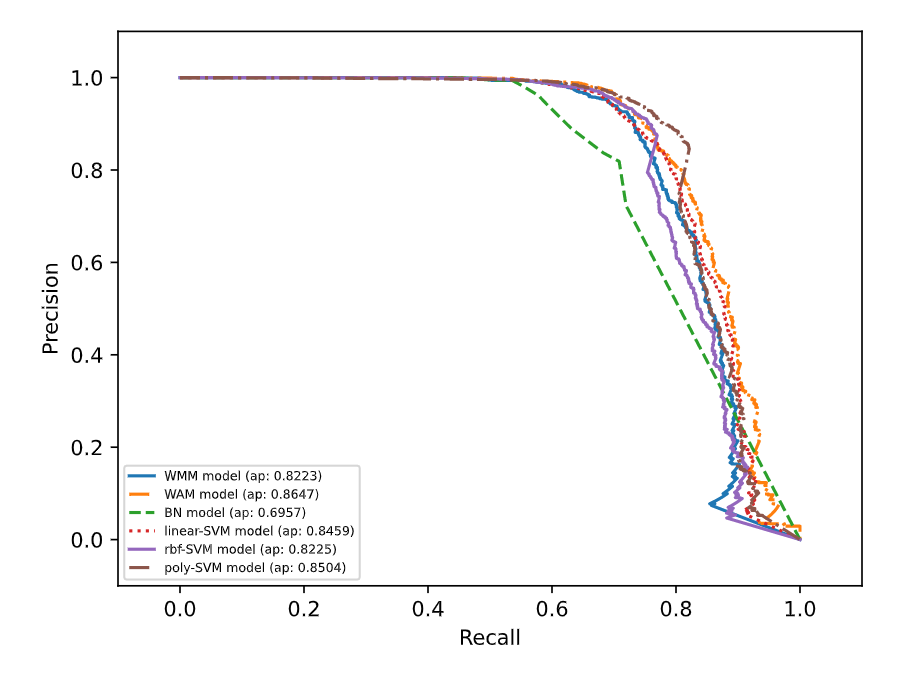
\includegraphics[scale=0.28]{Pics/all_prcurve_acceptor.png}
    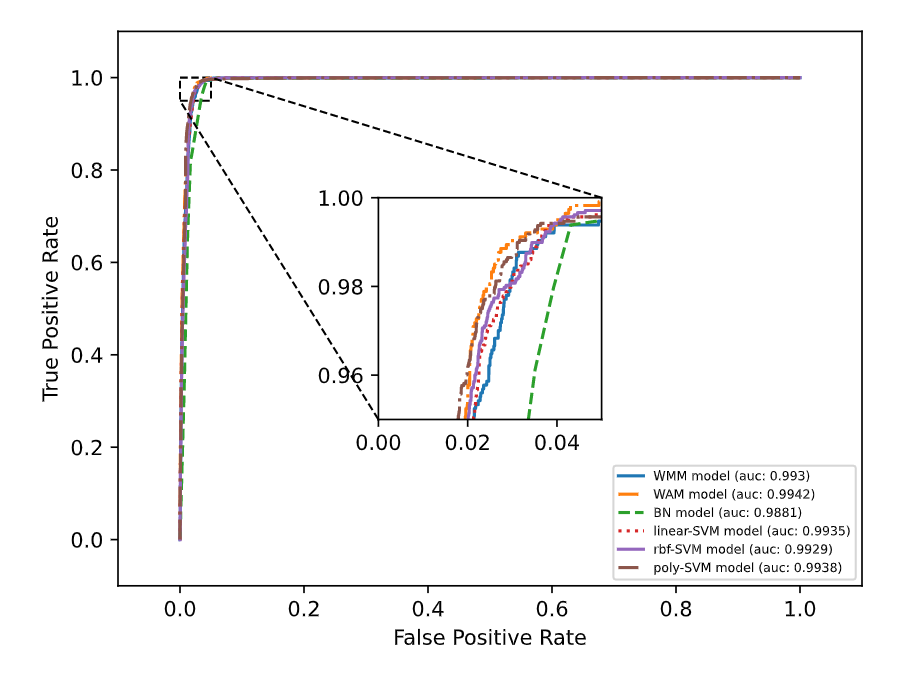
\includegraphics[scale=0.28]{Pics/all_roccurve_acceptor.png}}
\caption{Precision-Recall curves (\textbf{left}) and ROC curves (\textbf{right}) for acceptor signal. Bayesian network used for acceptor seems to have a lower predicting ability relative to the one for donor. }
\label{fig7}
\end{figure*}

\begin{figure}[htbp]
\centerline{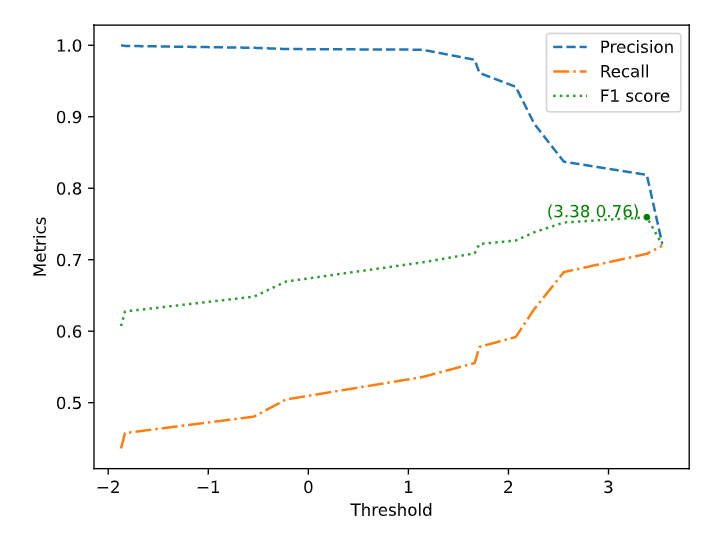
\includegraphics[scale=0.35]{Pics/BN_threshold_acceptor.png}}
\caption{Searching for the best threshold for acceptor prediction. We have found the maximum F1 point for BN: (3.38, 0.76). }
\label{fig8}
\end{figure}

\subsection{Donor Site Prediction}\label{4.2}

We compared the performance of various splice site predicting models such as WMM, WAM, SVM and the Bayesian network. The results shown in Fig. \ref{fig5} acknowledge that Bayesian network do not perform as good as expected, giving the proof that, under the same circumstances, it is more difficult for Bayesian models to learn the pattern of splice sites because of its sophisticated training steps, without any human intervention on the prior knowledge. It verifies that donor site prediction extremely relies on nothing but two conservative points shown in Fig. \ref{fig1}, whose strong impact on positive splice sites, however, is not paid attention by the network model. Chances are that the hyperparameters we set for the BN are not perfect, additionally, since we abandoned parameter grid searching thanks to its training time consumption. 

We present the stats of accuracy for all evaluated models in Table \ref{tab2}, in which the best threshold for BN is searched by F1-scoring (Fig. \ref{fig6}). 

\subsection{Acceptor Site Prediction}\label{4.3}

We did the same experiment on acceptor sites. Consequences are displayed in Fig. \ref{fig7} -- \ref{fig8} and Table \ref{tab3}. 


\begin{table*}[htbp]
\begin{center}
\begin{threeparttable}
\caption{Performance of BN Against Other Acceptor Site Predictors}
\begin{tabular}{lccccc}
\toprule
Method & Precision & Recall (TPR) & FPR & F1-score & Run time(s) \\
\midrule
WMM (threshold = 2.69) & 0.7385 & \textbf{0.9038} & 0.0160 & 0.8128 & \textbf{1.3336} \\
WAM (threshold = 2.54) & 0.7554 & \textbf{0.9038} & 0.0146 & 0.8229 & 1.4286 \\
Linear - SVM (threshold = 2.46) & 0.7603 & 0.8653 & 0.0137 & 0.8094 & 2.5636 \\
RBF - SVM (threshold = 2.40) & 0.7677 & 0.8999 & 0.0136 & 0.8285 & 4.6039 \\
4D poly - SVM (threshold = 2.55) & \textbf{0.7774} & 0.8975 & \textbf{0.0129} &  \textbf{0.8331} & 3.3924 \\
BN (threshold = 3.38) & 0.7083 & 0.8187 & 0.0169 & 0.7595 & 1.02e+3 \\
\bottomrule
\end{tabular}
\label{tab3}
\end{threeparttable}
\end{center}
\end{table*}

\section{Discussion}

Overall, we formulate and re-implement an application of Bayesian network model by training it on the Kulp \& Reese dataset. We find the best type \uppercase\expandafter{\romannumeral1} error to learn an appropriate DAG structure and compare its performance against other feasible approaches. Although no ideal results are given in this paper, we do not regard this as a failure. The availability for Bayesian networks on splice site prediction tasks is still proven in our work. 

As a matter of fact, there are still some blemishes in our methods which need to be taken serious consideration. For the preprocessing of the training set, we only sampled a fraction of data for model learning thus the network may not attain its best performance with the given dataset. We ignored the odds of base indels in signal sequences. We omitted unambiguous bases at the beginning of our work which is likely to be part of the splice site patterns. What's more, we only tried one single feature selection tactic limited by the deadline (our model is actually designed for feature sequences of different lengths as input). 

From the results above, a Bayesian network performs prediction at a pretty low speed (a reduction of one magnitude) compared to other models, for the massive computing of conditional probabilities. With the rapid development of high-throughput sequencing, promotion of predicting speed to match the sequencing is a matter of great concern nowadays, hence this is a serious problem for Bayesian methods. 

The network learning algorithms need an improvement. Even the most efficient constraint-based structural learning algorithms have a tremendous time complexity and are only suitable for sparse networks, that is, they are still unacceptable for predicting large functional sites with complicated interdependency, let alone the searching methods. 

Low robustness on unbalanced data. WAM and SVM shows eligible adaptability against training data with a partiality for negative samples but a Bayesian network does not. We found in our experiment that different ratios of positive and negative samples have a great impact on the performance of network because of the volatility of conditional probabilities of those variables. A characteristic of actual sequence data is the imbalance between positive and negative sites, the stability of pattern predictors against such data imbalance are accordingly in great demand. While the oversampling strategy works, as shown in our experiment, it lowers the generality of Bayesian networks and amplifies the noises mingled in the positive data. 

Despite the downside, Bayesian networks still have potential for predicting functional sites efficiently and accurately. In the future, we will dedicate ourselves to improving Bayesian networks in general. Several methods for structural and parametric learning will be applied and further evaluated for this task. We will also try to add more interference in the training process to assist the network in finding the right interdependency between variables. 

\section*{Acknowledgment}

This work was supported by Prof. Zhou from College of Life Science \& Technology, Huazhong University of Science and Technology, and Wuhan National Laboratory for Optoelectronics for providing computing resources. Also acknowledge our classmates for helpful suggestions \& corrections. 

\bibliographystyle{unsrt}
\bibliography{references}

\end{document}
